\newpage
\section{VL 03: Einfluss von IT-Systemen auf Geschäftsmodelle}

In dieser Vorlesung ging es hauptsächlich um die Veränderung eines Geschäftsmodells durch IT. Zunächst einmal wird der Markt für ein Produkt durch verschiedene Aspekte beeinflusst:

\begin{itemize}

    \item Substitute (d.h. Ersatzprodukte)

    \item Kundeneinfluss

    \item Lieferanteneinfluss

    \item Markteintritte (Neue Produkte / Unternehmen)

\end{itemize}

\subsection{Das Business Model Canvas}
    Um ein Geschäftsmodell besser beschreiben zu können, wurde das ,,Business Canvas Model'' eingeführt:

    \begin{center}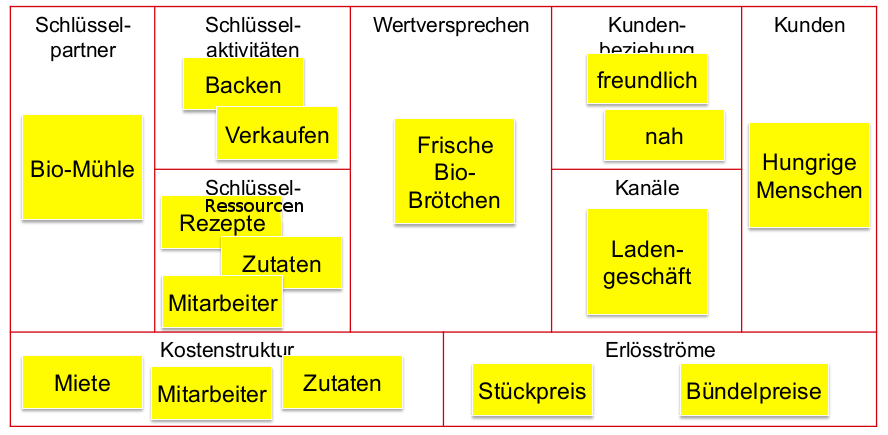
\includegraphics[width=1\textwidth]{BCM.png}\end{center}

    Die IT nimmt auf jeden der Aspekte im Diagramm auf verschiedene Arten und Weisen Einfluss:

    \begin{description}

        \item[Schlüsselpartner]
            Vereinfachte Einbindung von Partnern / digitale Partner (Suchmaschinen)

        \item[Schlüsselaktivitäten]
            Automatisierung / Beschleunigung / Tracking, Überwachung

        \item[Schlüsselressorucen]
            Information / Informationssysteme / Informations- und Kommunikations-Infrastruktur /
            (offene) It-Schnittstellen

        \item[Wertversprechen]
            Bessere Informationen und Kommunikation / Informationsbasierte Produkte \& Dienstleistungen /
            Günstigere, schnellere Leistungen

        \item[Kundenbeziehung]
            Websites / Applications / Selbstbedienung / Nutzergenerierte Inhalte / Communities

        \item[Kanäle]
            Electronic und Mobile Commerce / Intermediation: Etablierung eines neuen Mittlers.
            / Reintermediation: Erneute Etablierung eines Mittlers

        \item[Kunden]
            Veränderung von Zielgruppen etc. (auch international)

        \item[Erlösströme]
            Nutzungsabhängige Preise ("Pay-per-use") /
            Indirekte Erlöse (Daten verkaufen, Crapware installieren, Werbung)

        \item[Kostenstruktur]
            geringere Transaktionskosten / Vereinfachtes Verteilen von Risiken

    \end{description}

    Insgesamt werden Geschäftsmodelle durch IT umfangreich verändert, dabei geht es
    besonders um \textbf{Vermittlung und Koordination} von Dienstleistungen und Produkten,
    sowie um die Erschließung \textbf{neuer Partner} (viele kleine Anbieter).
